\documentclass{acm_proc_article-sp}

\usepackage{graphicx}% Include figure files
\usepackage{dcolumn}% Align table columns on decimal point
\usepackage{bm}% bold math
\usepackage{float}
\usepackage{array}
\usepackage{verbatim}
\usepackage{tikz}
\usepackage{hyperref}% add hypertext capabilities
\usepackage{xcolor}
%\usepackage[mathlines]{lineno}% Enable numbering of text and display math
%\linenumbers\relax % Commence numbering lines
%\usepackage[section]{placeins}
\usepackage{caption}
\usepackage{subcaption}


\usepackage{listings}
%\usepackage{footnote}
%\makesavenoteenv{table}
%\makesavenoteenv{table*}
%\makesavenoteenv{tabular}

\begin{document}

\title{Self-Organizing systems WS14\\
       Hexagonal SOM extention}

\numberofauthors{2}
\author{
Richard Plangger\\
\email{e1025637@student.tuwien.ac.at}
\alignauthor
Rene Koller\\
\email{eXXXXXXX@student.tuwien.ac.at}
\alignauthor
}

\date{\today}

\maketitle

\begin{abstract}
    This document describes our solution to the assignment
    to extend the SOM Toolbox to train and display a hexagonal
    SOM
\end{abstract}

\keywords{Self organizing systems, SOM, hexagonal, training}

\section{SOM Toolbox}

For this assignment we used the SOM Toolbox~\cite{somtoolbox}. Our solution
is based on the source code found in the section ``Download Latest'' and is
identified by the version ``0.7.5-4.svn4332''.

\section{Terminology}

As shown in Figure~\ref{fig:coord} both hexagonal and rectangular
use the same coordinate system to reference nodes from their memory.
There was no need to modify the array cell layout, but only adjust the
calculation for the grid neighbours. The major
difference while using hexagonal grid system is that there are not only
four direct neighbours but six.

The neighbours using $(X/Y)$ as coordinate indices of $(1/1)$ in Figure~\ref{fig:coord-rect}
are $\{(1/2),(2/1),(1/0),(0/1)\}$. In Figure~\ref{fig:coord-hex} they are $\{(1/2),(2/2),(2/1),(2/0),(1/0),(0/1)\}$.

The hexagonal grid is rendered ``pointy top''\footnote{The hexagon is rotated in such a way that an edge points up} and every second row is shifted half width of a
cell to the left.

\begin{figure}
    \begin{subfigure}{1\linewidth}
    \centering
    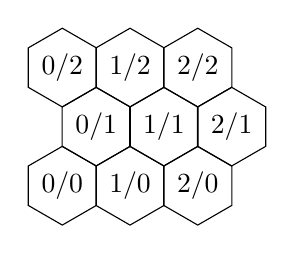
\begin{tikzpicture}
        \foreach \off / \x / \y in {0/0/0,0/1/0,0/2/0,0.43cm/0/1,0.43cm/1/1,0.43cm/2/1,0/0/2,0/1/2,0/2/2} {
            \draw ({\off + \x*0.86cm},{0.75cm * \y}) -- ++(30:0.5cm)
              \foreach \r in {90,150,210,270,330} { -- ++(\r:0.5cm) }
              -- cycle;
          \draw ({\off + \x*0.86cm},{0.75cm * \y + 0.5cm}) node {\x/\y};
        };
    \end{tikzpicture}
    \caption{hexagonal}
    \label{fig:coord-hex}
    \end{subfigure}

    \begin{subfigure}{1\linewidth}
        \centering
    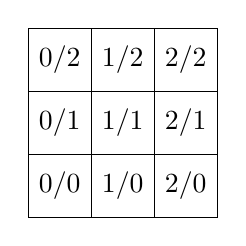
\begin{tikzpicture}
        \foreach \off / \x / \y in {0/0/0,0/1/0,0/2/0,0.43cm/0/1,0.43cm/1/1,0.43cm/2/1,0/0/2,0/1/2,0/2/2} {
            \draw ({0.8cm * \x},{0.8cm * \y})
              -- ++({0.8cm},{0})
              -- ++({0},{0.8cm})
              -- ++({-0.8cm},{0})
              -- cycle;
          \draw ({\x*0.8cm + 0.4cm},{0.8cm * \y + 0.4cm}) node {\x/\y};
        };
    \end{tikzpicture}
    \caption{rectangular}
    \label{fig:coord-rect}
    \end{subfigure}
    \caption{Coordinate system and layout}
    \label{fig:coord}
\end{figure}

To abstract the grid neighbourhood, geometric layout and rendering from the actual 3d \lstinline!Unit! array
representation a new interface has been introduced. The interface \lstinline!GridGeometry! is the base abstraction
to be able to calculate shapes, center of the shapes and the grid neighbours.

\section{Hexagonal Training}

By examining the training process implemented in \lstinline!GrowingLayer! we have identified the following two strategies.
First there is the single threaded training calculating the neighbourhood using the function presented in the lecture:
\[
    h_{ci} = \alpha \times exp(-\frac{dist(winner,unit)^2}{2\sigma^2})
\]
In the function \lstinline!updateUnitsInArea! $h_{ci}$ is the used to updated the weight vectors for each unit.

The second strategy is called batch SOM that, similar to the first stratgey, uses the squared distance to the neighbours
to mark the activation. It then updates the weight vector of every node by assigning the mean value of all mapped input
data samples in the neighbourhood.

Since the algorithms are so similar we decided not to duplicate the SOM training code contained in \lstinline!GrowingLayer! but
rather just abstract the distance measures. Both strategies mentioned earlier soley rely on the distance measure in the grid geometry.
Figure~\ref{fig:hci-coord-rect} illustrates the rectangular distance measurement.
The inner dashed circle has an euclidean distance of $\sqrt{1} = 1$ to
the unit center at position $(1,1)$. The geometry layout in the code does not calculate the distance from the center of
the unit square, but from the corner (lower left). The distance for the second dashed circle has an euclidean distance of $\sqrt(2) \approx 1.14$ and finally the last cirle has a distance from the unit (1/1) of $\sqrt{4} = 2$.

To achieve the same distances in a hexagonal grid our approach is visualized in Figure~\ref{fig:hci-coord-hex}.
The inner circle has a distance of $\sqrt{1} = 1$ to all of his 6 neighbours. To achieve this distance metric 
we use the rectangular unit space which with an unit $u$ from any neighbouring unit. Since the hexagon grid forces deformation
of the shapes the following forumlas are used to calculate the grid.

\begin{itemize}
    \item Hexagonal width using a reference unit $u$ (e.g cm)
        $ h_w(u) = u; h_w(1) = 1 $
    \item Hexagonal height using a reference unit $u$ \\
        $ h_h(u) = u \times \frac{2}{\sqrt{3}} * \frac{3}{4}; h_h(1) \approx 0.86 $
    \item Hexagonal shift using a reference unit $u$ \\
        $ h_s(u) = \frac{h_w(u)}{2}; h_s(1) = 0.5 $ \\
        Note that the hexagonal shift only returns a non zero
        value for every second row.
    \item Euclidean distance formula. 
    \begin{align*}
        d(p_1,p_2) & = \sqrt{ A^2 + B^2 }\\
        A & = (h_w(1) * p_2.x + h_s(1)) \\
          &- (h_w(1) * p_1.x + h_s(1))\\
        B & = (h_h(1) * p_2.y) - (h_h(1) * p_1.y)
    \end{align*}
    $p_x$ is a point in the rectangular grid. The dot-operator $x$ and $y$
    (e.g. $p_1.x$) get the rectangular position. Thus $d(p_1,p_2)$ is just the
    euclidean distance adjusted by the hexagonal shape width and height
    and every second row shifted by half of the width.
\end{itemize}

\colorlet{c1}{red}
\colorlet{c2}{violet}
\colorlet{c3}{cyan}

\begin{figure}
    \begin{subfigure}{1\linewidth}
    \centering
    \begin{tikzpicture}
        \foreach \off / \x / \y in {0/0/0,0/1/0,0/2/0,0/3/0,
                         0.43cm/0/1,0.43cm/1/1,0.43cm/2/1,0.43cm/3/1,
                         0/0/2,0/1/2,0/2/2,0/3/2,
                         0.43cm/0/3,0.43cm/1/3,0.43cm/2/3,0.43cm/3/3} {
            \draw ({\off + \x*0.86cm},{0.75cm * \y}) -- ++(30:0.5cm)
              \foreach \r in {90,150,210,270,330} { -- ++(\r:0.5cm) }
              -- cycle;
          \draw ({\off + \x*0.86cm},{0.75cm * \y + 0.5cm}) node {\x/\y};
        };

        \draw [fill,black] ({0.86cm * 1 + 0.43cm},{0.75cm * 1 + 0.5cm}) circle [radius=0.06cm];

        \draw [dashed,c1] ({0.86cm * 1 + 0.43cm},{0.75cm * 1 + 0.5cm}) circle [radius=0.86cm];
        \draw [dashed,c2] ({0.86cm * 1 + 0.43cm},{0.75cm * 1 + 0.5cm}) circle [radius={0.75cm * 2}];
        \draw [dashed,c3] ({0.86cm * 1 + 0.43cm},{0.75cm * 1 + 0.5cm}) circle [radius={2.2821cm}];
        \foreach \off / \x / \y in {0/1/0,0/2/0,0.43cm/0/1,0.43cm/2/1,0/1/2,0/2/2} {
            \draw [fill,c1] ({\off + 0.86cm * \x},{0.75cm * \y + 0.5cm}) circle [radius=0.06cm];
        };
        \foreach \off / \x / \y in {0/0/0,0/0/2,0/3/2,0/3/0,0.43cm/1/3} {
            \draw [fill, c2] ({\off + 0.86cm * \x},{0.75cm * \y + 0.5cm}) circle [radius=0.06cm];
        };
        \draw [fill,c3] ({0.43cm + 0.86cm * 3},{0.75cm * 3 + 0.5cm}) circle [radius=0.06cm];
    \end{tikzpicture}
    \caption{hexagonal}
    \label{fig:hci-coord-hex}
    \end{subfigure}

    \begin{subfigure}{1\linewidth}
        \centering
    \begin{tikzpicture}
        \foreach \off / \x / \y in {0/0/0,0/1/0,0/2/0,0.43cm/0/1,0.43cm/1/1,0.43cm/2/1,0/0/2,0/1/2,0/2/2} {
            \draw ({0.8cm * \x},{0.8cm * \y})
              -- ++({0.8cm},{0})
              -- ++({0},{0.8cm})
              -- ++({-0.8cm},{0})
              -- cycle;
          \draw ({\x*0.8cm + 0.4cm},{0.8cm * \y + 0.4cm}) node {\x/\y};
        };

        \draw [dashed,c1] ({0.8cm * 1},{0.8cm * 1}) circle [radius=0.8cm];
        \draw [fill,c1] ({0.8cm * 1},{0.8cm * 0}) circle [radius=0.06cm];
        \draw [fill,c1] ({0.8cm * 0},{0.8cm * 1}) circle [radius=0.06cm];
        \draw [fill,c1] ({0.8cm * 2},{0.8cm * 1}) circle [radius=0.06cm];
        \draw [fill,c1] ({0.8cm * 1},{0.8cm * 2}) circle [radius=0.06cm];

        \draw [fill,black] ({0.8cm * 1},{0.8cm * 1}) circle [radius=0.06cm];

        \draw [dashed,c2] ({0.8cm * 1},{0.8cm * 1}) circle [radius={1.1313cm}];
        \foreach \x / \y in {0/0,2/0,2/2,0/2} {
            \draw [fill,c2] ({0.8cm * \x},{0.8cm * \y}) circle [radius=0.06cm];
        }

        \draw [dashed,c3] ({0.8cm * 1},{0.8cm * 1}) circle [radius={0.8cm * 2}];
        \foreach \x / \y in {3/1,1/3} {
            \draw [fill,c3] ({0.8cm * \x},{0.8cm * \y}) circle [radius=0.06cm];
        }
    \end{tikzpicture}
    \caption{rectangular}
    \label{fig:hci-coord-rect}
    \end{subfigure}
    \caption{Coordinate system and layout}
    \label{fig:coord}
\end{figure}

\bibliography{ref}
\bibliographystyle{plain}

\end{document}
